%\documentstyle[epsf,twocolumn]{jarticle}       %LaTeX2.09仕様
%\documentclass[twocolumn]{jarticle}     %pLaTeX2e仕様
\documentclass{jarticle}     %pLaTeX2e仕様

%一枚組だったら[twocolumn]関係のとこ消す

\setlength{\topmargin}{-45pt}
%\setlength{\oddsidemargin}{0cm} 
\setlength{\oddsidemargin}{-7.5mm}
%\setlength{\evensidemargin}{0cm} 
\setlength{\textheight}{24.1cm}
%setlength{\textheight}{25cm} 
\setlength{\textwidth}{17.4cm}
%\setlength{\textwidth}{172mm} 
\setlength{\columnsep}{11mm}

\kanjiskip=.07zw plus.5pt minus.5pt

\usepackage[dvipdfm]{graphicx}
\usepackage{ccaption}
\usepackage{algorithm}
\usepackage{algorithmic}
\usepackage{subcaption}
\usepackage{enumerate}
\usepackage{comment}
\usepackage{url}
\usepackage{multirow}
\usepackage{diagbox}
\usepackage{amssymb}
\usepackage{mathtools}
\usepackage{wrapfig}
\usepackage{graphicx}
\usepackage{float}
\usepackage{amsmath}
\usepackage{lipsum}


\begin{document}
  \noindent
  \hspace{1em}

  \today Creation班 ゼミ
  \hfill
  \ \  西村昭賢 

  \vspace{2mm}
  \hrule
  \begin{center}
  {\Large \bf 進捗報告}
  \end{center}
  \hrule
  \vspace{3mm}


\section{やろうとしていたこと}
ダ鳥獣ギ画\cite{sozai}のカエルのような画風の 3D モデルを Text to 3D 手法を用いて生成する.

\section{用いたText to 3D 手法}
DreamFusionc\cite{poole2022dreamfusion} を用いた.
深層学習を用いて様々な画像から 3D シーンを生成する NeRF \cite{NeRF}, Text to Image 手法の Imagen\cite{Imagen} に加えて拡散モデルを利用している.
図 \ref{fig:DreamFusion} に Dream Fusion の概略を示す. 

\begin{figure}[ht]
  \centering
  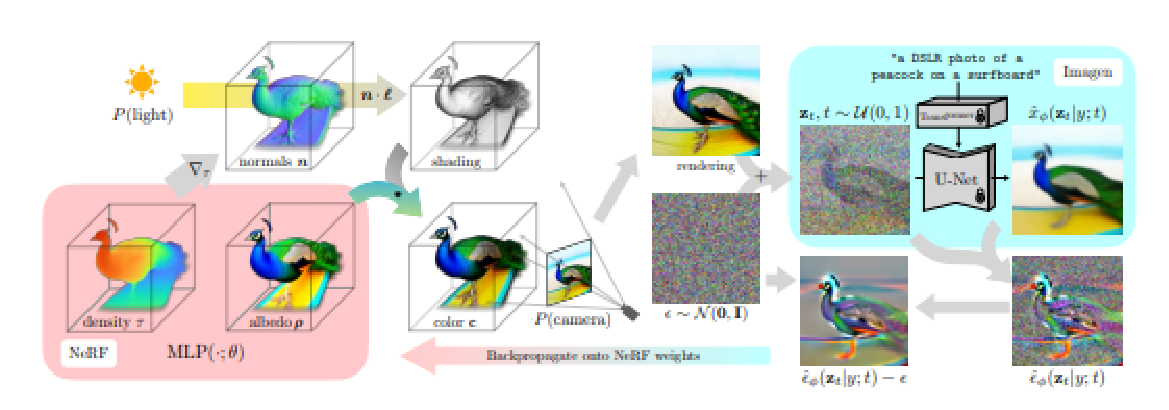
\includegraphics[width=120mm]{assets/dreamfusion.eps}
  \vspace{-0.3cm}
  \caption{DreamFusion 概略図}
  \label{fig:DreamFusion}
\end{figure}

\section{下準備}
ダ鳥獣ギ画のカエルの画風の Text to Image モデルを用意する必要がある. 
今回は, Stable Diffusion のファインチューニング手法として Text Inversion\cite{TextInversion} を用いた.
図 \ref{fig:beforeFT} にファインチューニング前のモデルに "an illustration of flog" というプロンプトを与えた際に生成された画像, 図 \ref{fig:AfterFT} にファインチューニング後のモデルに "an 	\textless giga-style \textgreater illustration of flog" というプロンプトを与えた際に生成された画像を示す.
ダ鳥獣ギ画っぽい画風で生成できていることが分かる.
\begin{figure}[ht]
  \centering
  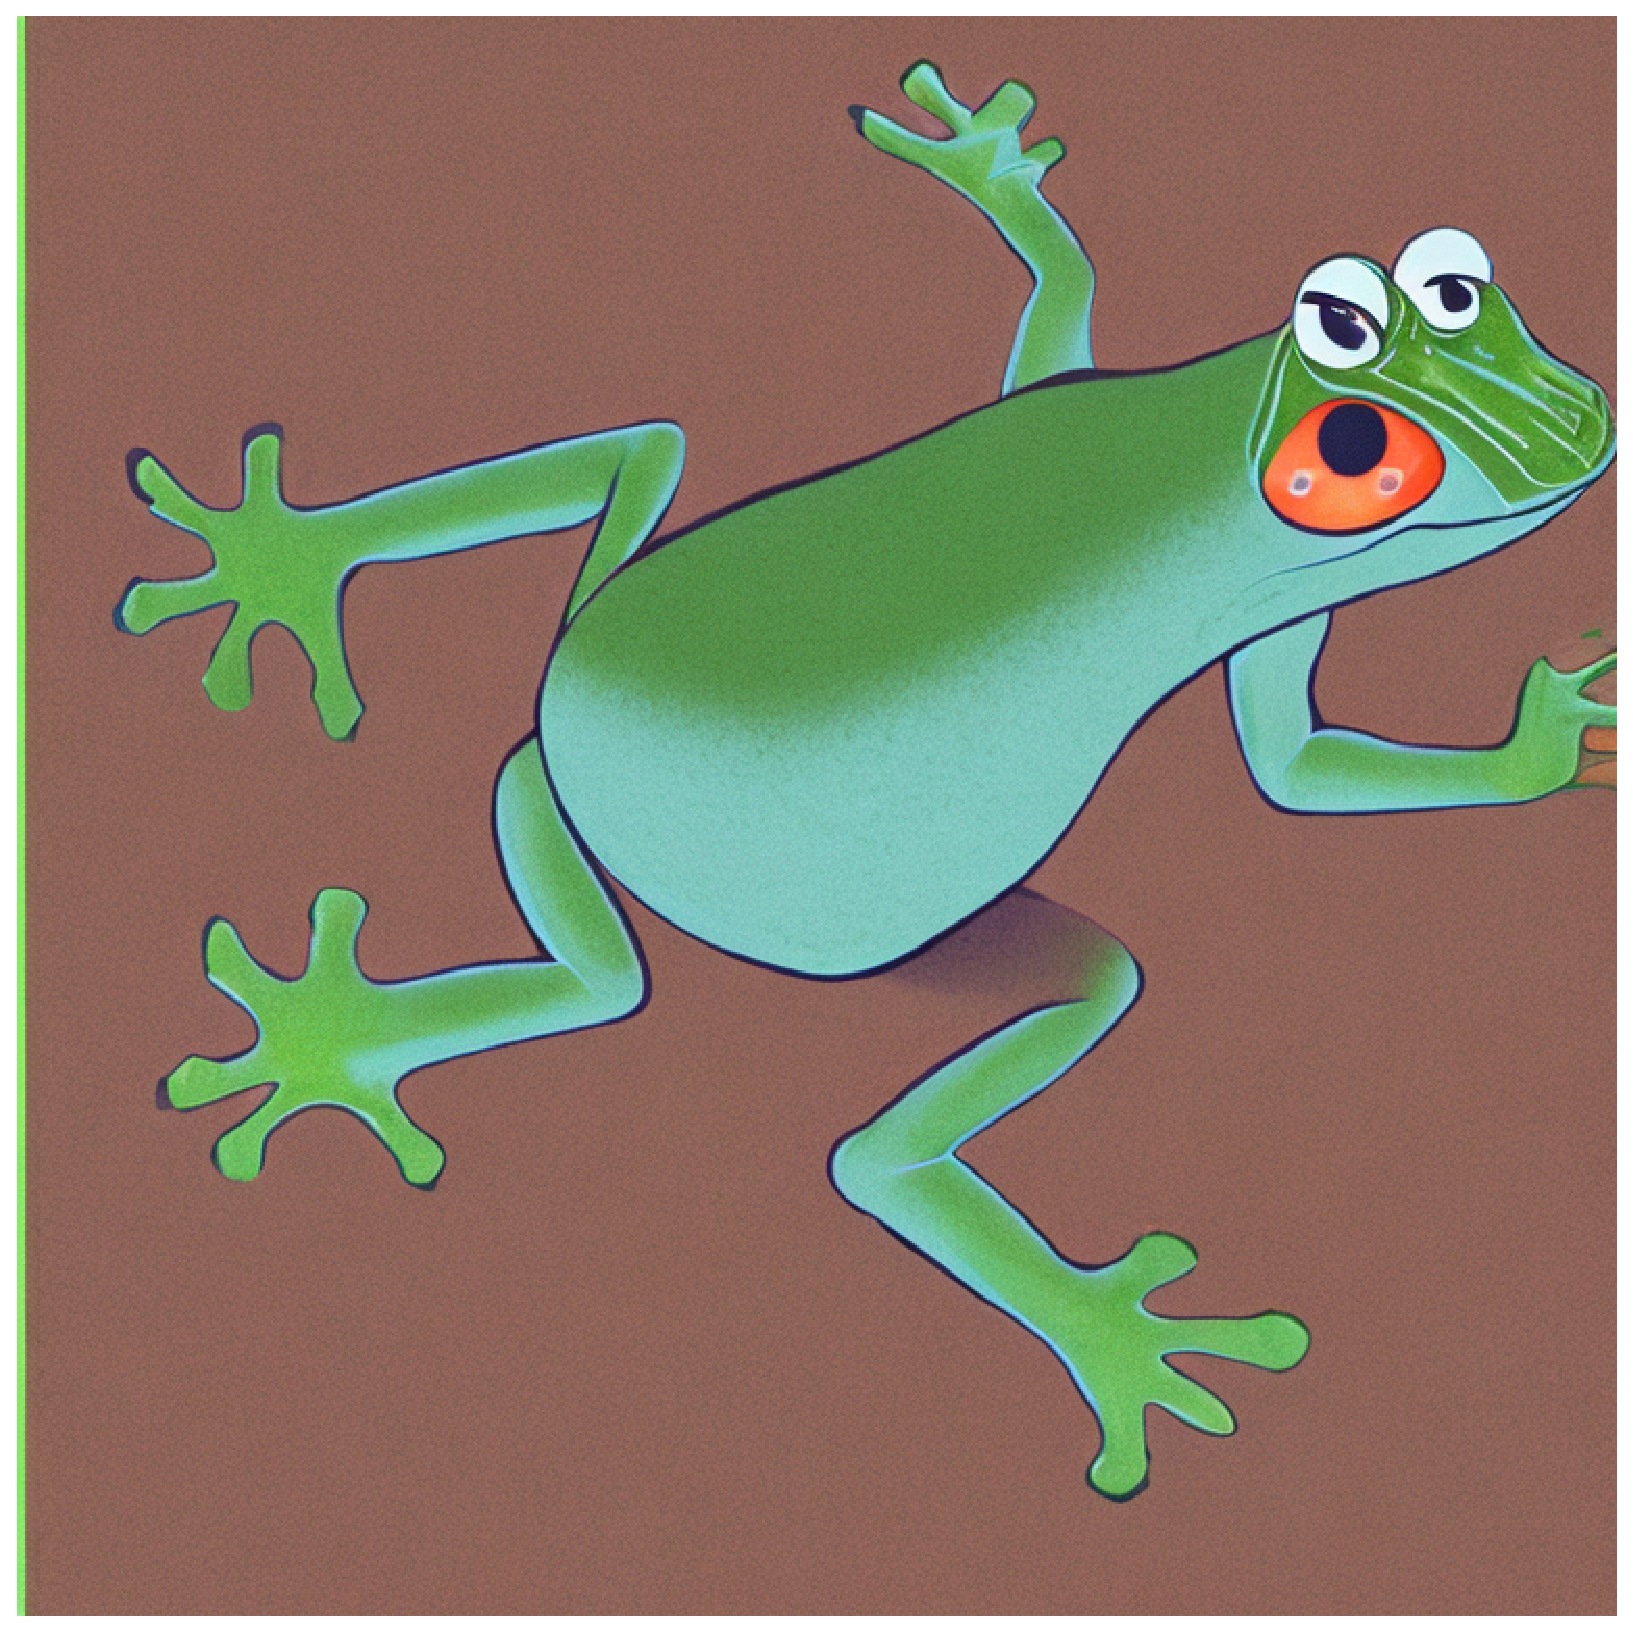
\includegraphics[width=120mm]{assets/beforeFT.eps}
  \vspace{-0.3cm}
  \caption{DreamFusion 概略図}
  \label{fig:beforeFT}
\end{figure}

\begin{figure}[ht]
  \centering
  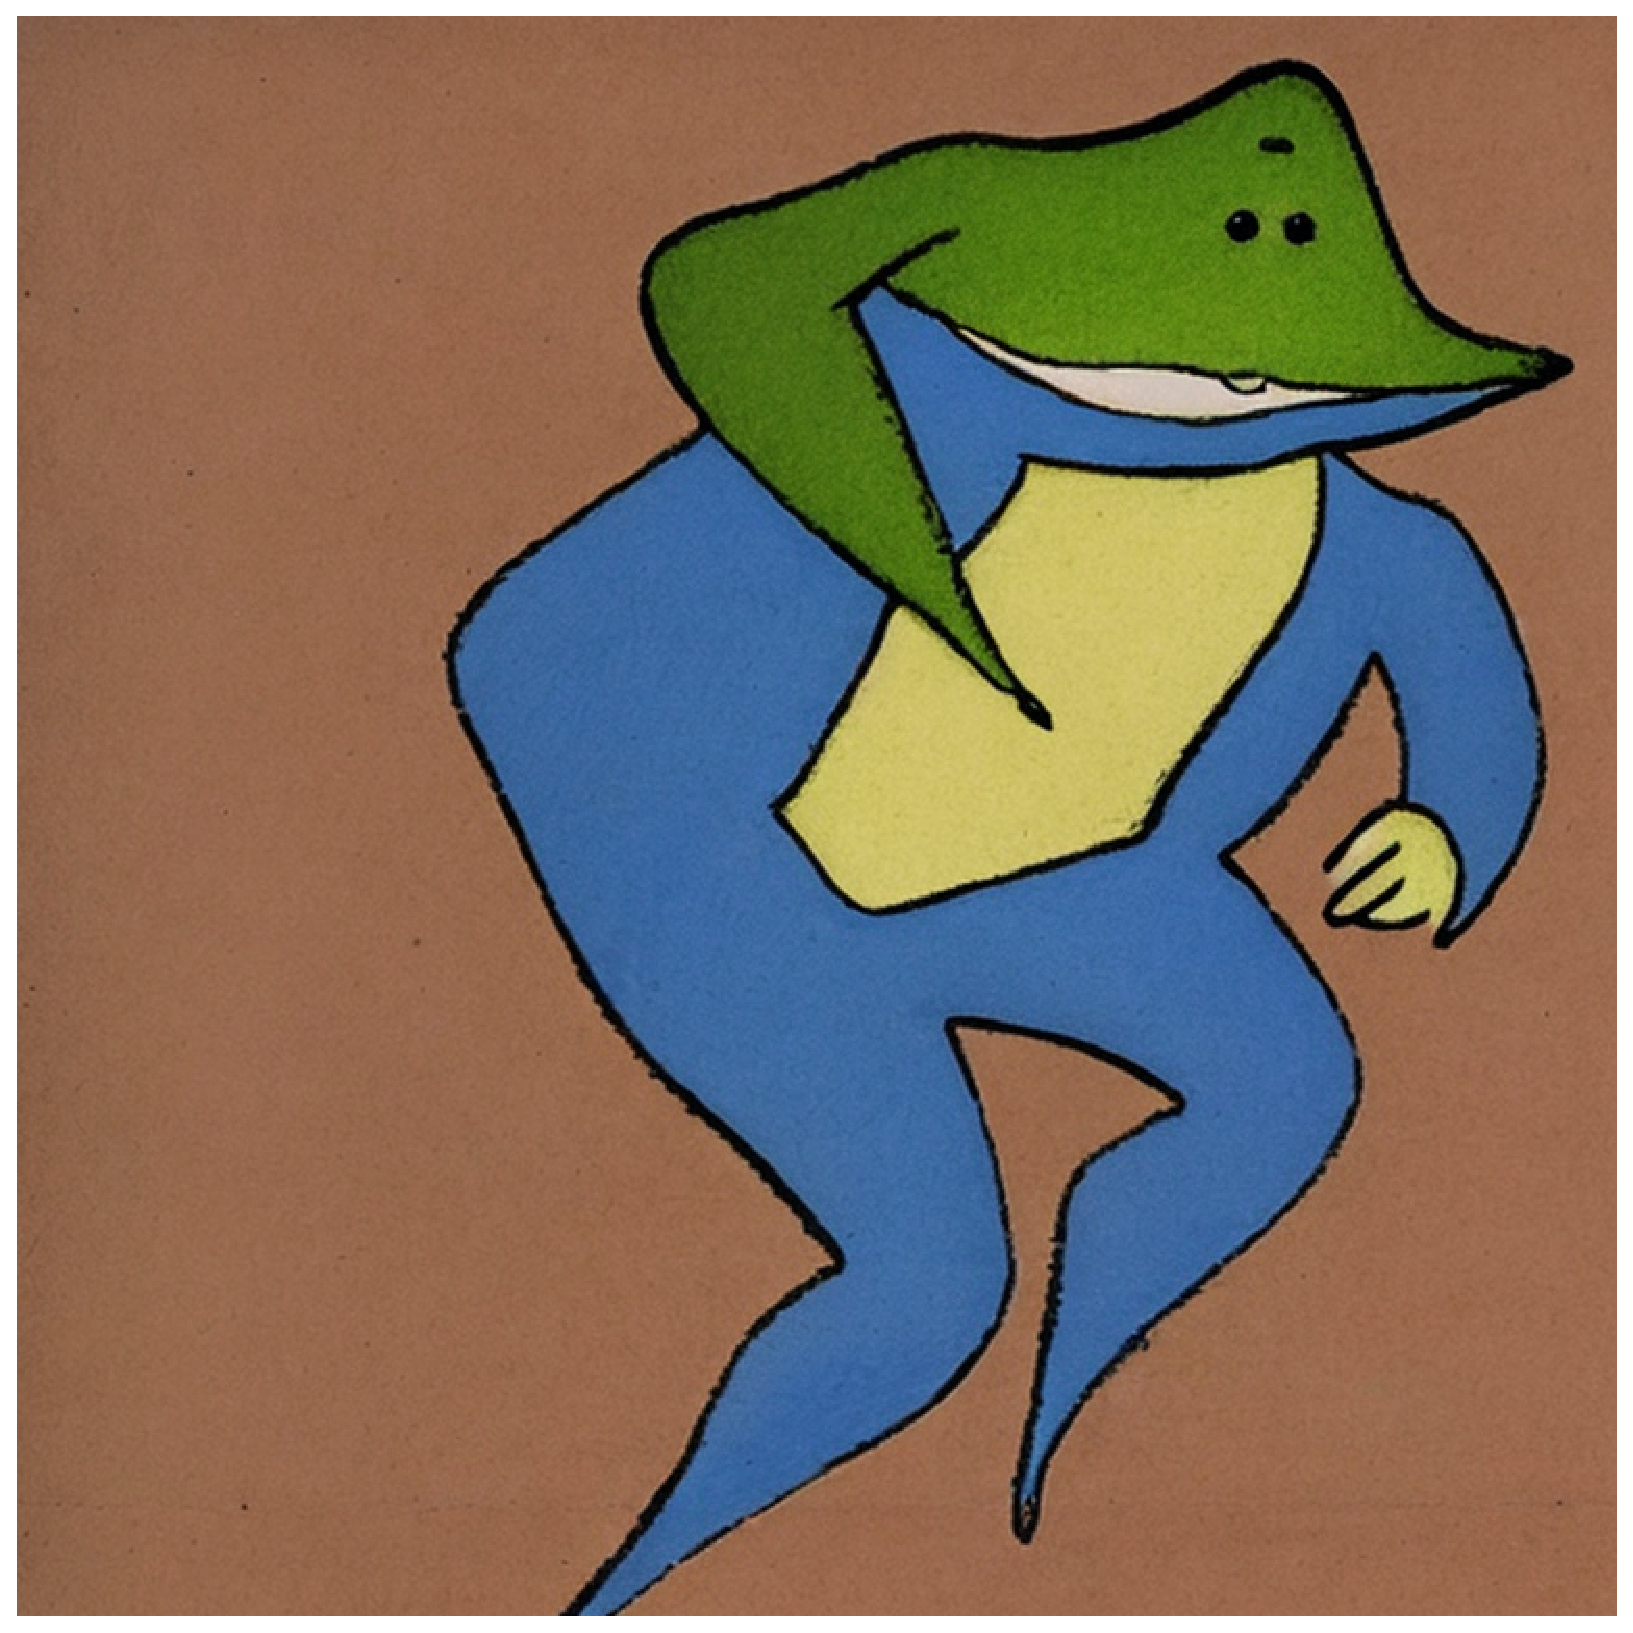
\includegraphics[width=120mm]{assets/AfterFT.eps}
  \vspace{-0.3cm}
  \caption{DreamFusion 概略図}
  \label{fig:AfterFT}
\end{figure}


\section{Text to 3D}
READMEに従って 100 エポックほど学習しようとしたところ, 実験で用いていた aiserv では 20 エポック時点で cuda out of memory error が出てしまい, 十分に学習が進まなかった.
20エポック時点(学習が止まった段階) の動画があるため, それを流します. 
FT 前はもちろん, FT 後の拡散モデルを用いた場合でもカエルっぽい概形はできているが, FT 後の拡散モデルを用いて生成したモデルがダ鳥獣ギ画の画風を反映しているとは現時点では言えない.

\section{課題}
\begin{itemize}
  \item 研究の方向性
  \item マシンスペック
  \par
  DreamFusion のレポジトリの issue を見ていると GPU のメモリが最低 12GB 必要らしい. aiserv の GPU(Geforce RTX 3070) は 8GB だったため実験が途中で終わったと考えられる.

\end{itemize}


%index.bibはtexファイルと同階層に置く
%ちゃんと\citeしないと表示されない(1敗)
\bibliography{index.bib}
\bibliographystyle{junsrt}

\end{document}